\documentclass[a4paper,11pt]{article}
\usepackage[utf8]{inputenc}
\usepackage[T1]{fontenc}
\usepackage{babel}

% font
\usepackage{amsmath}
\usepackage{amsfonts}
\usepackage{amssymb}
% marges
\usepackage{vmargin}
% en-tete
\usepackage{fancyhdr}
% indice en mode texte
\usepackage{subscript}
% symbole euro
\usepackage{marvosym}
% faire des graphes, arbres
\usepackage{tikz}
\usetikzlibrary{positioning,shadows,arrows}
% pour les boucles for
\usepackage{pgffor}
% pour les traits sous les sections
\usepackage{sectsty}
% pour les tableaux
\usepackage{array}
\usepackage{multirow}
\usepackage[table]{xcolor, colortbl}
% augmenter l'interligne
\usepackage{setspace}
% justifier le texte
\usepackage{ragged2e}


% images
\usepackage[pdftex]{graphicx}
\usepackage{subfig} 
\usepackage{caption}
\usepackage{subcaption}
\usepackage{wrapfig}
\setlength{\headheight}{15pt} % supprime un warning

% insertion de code source
\usepackage{listings}
\definecolor{colKeys}{rgb}{0,0,1} 
\definecolor{colIdentifier}{rgb}{0,0,0} 
\definecolor{colComments}{rgb}{0,0.5,1} 
\definecolor{colString}{rgb}{0.6,0.1,0.1} 
\lstset{
    language=C,
    basicstyle=\ttfamily\small, % 
    identifierstyle=\color{colIdentifier}, % 
    keywordstyle=\color{colKeys}, % 
    stringstyle=\color{colString}, % 
    commentstyle=\color{colComments}, % 
    % identifierstyle=ttfamily,
    showstringspaces=false,
    numbers=left,
    stepnumber=1,
    numbersep=10pt,
    tabsize=2,
    breaklines=true,
    breakatwhitespace=false,
    columns=fixed,
    extendedchars=true
}
% Pour afficher des algos
\usepackage[french,onelanguage,lined,boxed]{algorithm2e}

% police
\newcommand\code[1]{\shorthandoff{:}{\texttt{#1}}}
\newcommand\titlefont[2]{{\fontfamily{phv}\fontsize{#1}{11pt}\selectfont #2}}

%couleur
\usepackage{color}
%%% based on official palette for internship presentations
\definecolor{utbmpurple}{RGB}{125,92,139}
\definecolor{utbmyellow}{RGB}{242,227,146}
\definecolor{utbmgreen}{RGB}{217,217,87}
\definecolor{utbmgrey}{RGB}{128,128,128}
\definecolor{utbmgreybandeau}{RGB}{79,78,85}
\definecolor{utbmwtfisthatpink}{RGB}{184,80,93}
\newcommand{\boitecolor}[3]
   {\colorbox{#1}{\textcolor{#2}{#3}}}

% marges
%%%% debut macro %%%%
\newenvironment{changemargin}[2]{\begin{list}{}{%
\setlength{\topsep}{0pt}%
\setlength{\leftmargin}{0pt}%
\setlength{\rightmargin}{0pt}%
\setlength{\listparindent}{\parindent}%
\setlength{\itemindent}{\parindent}%
\setlength{\parsep}{0pt plus 1pt}%
\addtolength{\leftmargin}{#1}%
\addtolength{\rightmargin}{#2}%
}\item }{\end{list}}
%%%% fin macro %%%%
% ligne horizontale
\newcommand{\HRule}{\rule{\linewidth}{0.5mm}}
% format de numerotation des sections / subsections
% \renewcommand\thesection{\Roman{section}}
% \renewcommand{\thesubsection}{\Alph{subsection}}
% \renewcommand{\thesubsubsection}{\arabic{subsubsection}}

\newcommand{\letitre}{LO53 : Positioning system} 
\title{\letitre}
\author{Antoine \textsc{Gréa}, Florentin \textsc{Toulemon}}
\date{\today}


\begin{document}

    \begin{titlepage}
    \setmarginsrb{0mm}{0mm}{0mm}{0mm}{0pt}{0mm}{12pt}{12mm}
    % trim = l b r t (l from the left, b from the bottom, r from the right, and t from the top)
    \noindent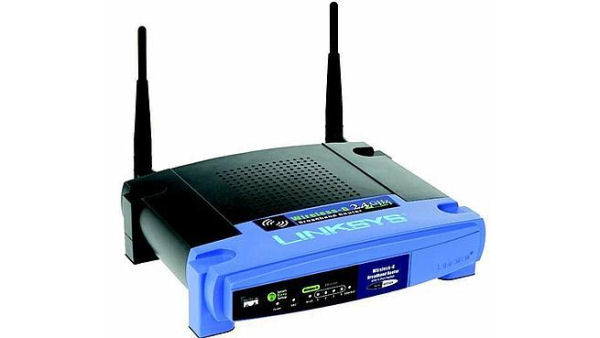
\includegraphics[clip,width=\textwidth,height=10cm]{images/baniere.jpg}
    \vspace{-1px}
    \noindent\boitecolor{black}{white}{
    \makebox[\textwidth][l]{\hspace{1cm}\titlefont{14}{
    \textbf{UNIVERSITÉ DE TECHNOLOGIE} DE BELFORT-MONTB\'ELIARD}}}
    \vspace{-1px}
    \noindent\boitecolor{utbmpurple}{white}{
    \makebox[\textwidth][l]{\hspace{1cm}\titlefont{22}{
    \textbf{\letitre}}}}
    \vspace{-1px}
    \noindent\boitecolor{utbmgreybandeau}{white}{
    \makebox[\textwidth][l]{\hspace{1cm}\titlefont{14}{
        Rapport de LO53 - P2012}}}

\noindent\fcolorbox{utbmgreen}{utbmgreen}{
\begin{minipage}{\textwidth}
    \vspace{1cm}\hspace{0.5cm}
    \begin{minipage}{0.75\textwidth}
        \begin{flushleft} \titlefont{18}{
            \textbf{\textsc{Gréa} Antoine}\\
            \vspace{0.1cm}
            \textbf{\textsc{Toulemon} Florentin}}\\
            \vspace{0.1cm}
            \titlefont{14}{
            \textbf{Génie Informatique}}
        \end{flushleft}
    \end{minipage}
    
    \vspace{1cm}\hspace{0.5cm}
    \begin{minipage}{0.5\textwidth}
        \begin{flushleft} \titlefont{14}{\textcolor{utbmgrey}{
            Suiveur UTBM}}\\
            \vspace{0.1cm}
            \titlefont{18}{
            \textbf{\textsc{Lassabe} Frédéric}}
        \end{flushleft}
    \end{minipage}
    \vspace{6.6cm}
\end{minipage}}

    \vspace{0.2cm}
    \noindent\boitecolor{white}{white}{\makebox[\textwidth][l]{
        \begin{minipage}{0.9\textwidth}
            \begin{flushright}
                
\includegraphics[width=4cm]{images/utbmlogo.jpg}
            \end{flushright}
        \end{minipage}
    }}

\enlargethispage{5cm}

\end{titlepage}
\pagecolor{white}


    \newpage
    \pagestyle{fancy}
    \pagenumbering{arabic} \setcounter{page}{2}
    \lhead{}
    \rhead{LO53 - P2012}
    \lfoot{A. \textsc{Gréa} - F. \textsc{Toulemon}}
    \rfoot{
\includegraphics[width=1cm]{images/utbmlogo.jpg}}
    \cfoot{\shortstack{\thepage \\ 
        \raisebox{-0.5cm}{\tiny\textcolor{utbmgrey}{
            \shortstack{\propriete}}}
        }
    }
    \enlargethispage{-5cm}
    \tableofcontents
    \newpage
    \lhead{Introduction}
\section*{Introduction}


\foreach \n in {1,...,4}
{
    \include{includes/part\n}
}

\lhead{Conclusion}
\section{Conclusion}

This project was very interesting because it gave us the opportunity to work on
several parts of the indoor positioning mechanism.

We increased our programing skills in Java, SQL and C. Also, we could create an
Android application and a server, introducing ourselves to servlet development
and tomcat server.



    \newpage

\end{document}
